% !TEX root = sample.tex
%%==========================================================================
\section{SuperMatching}
\label{sec:supersymhopm}
%-------------------------------------------------------------------------
We now discuss the first and second issues mentioned above, which are independent of application; later we turn to definition of affinity measure, which is application dependent, and sampling strategy.

\subsection{Supersymmetric affinity tensor}
\label{subsec:supersymtensor}

A tensor generalises vectors and matrices to higher dimensions: a vector is a tensor of order one,
and a matrix is a tensor of order two. A higher-order tensor can be expressed as a multi-dimensional array~\cite{Kolda08}.
Here we consider a higher-order supersymmetric affinity tensor, which represents a real-valued higher-order affinity between feature tuples.

\newtheorem{mot}{Definition}
\begin{mot}[Supersymmetric Tensor]
\label{mot:def1}
A tensor is called supersymmetric if its entries are invariant under any permutation of its indices~\cite{Kofidis02}.
\end{mot}

For example, a third-order supersymmetric tensor $\mathcal{T}_3$, satisfies the relationships:
$\mathcal{T}_3(i_1, i_2, i_3)=\mathcal{T}_3(i_1, i_3, i_2)=\mathcal{T}_3(i_2, i_1, i_3)=\mathcal{T}_3(i_2, i_3, i_1)=\mathcal{T}_3(i_3, i_1, i_2)=\mathcal{T}_3(i_3, i_2, i_1)$.

Consider $T_N(i_1,\cdots,i_N)$, in Equ.(\ref{equ:assigment}), which measures the affinity of the assignments $(i_1,  \cdots, i_N)$; in other words it  uses the value $\phi_N(i_1,\cdots, i_N)$
%%%RRM First write some stuff to say if phi IS the affinity, or if not, how it is related to it.
to give a score when matching the ordered feature tuple $(i^{'}_1,\cdots,i^{'}_N)$ from $P_1$ to the ordered feature tuple $(j^{'}_1,\cdots,j^{'}_N)$ from $P_2$,.
Often, the value of $\phi_N(i_1,  \cdots, i_N)$ is invariant under permutation of its arguments $(i_1, \cdots, i_N)$.
%%%RRM Give a simple example?
%for example, see the third-order potential function $\phi_3$ used in~\cite{Duchenne_etal09,Chertok10}.
Obviously, a higher-order supersymmetric tensor $\mathcal{T}$ can be used to capture this information:
\begin{mot}[Supersymmetric Affinity Tensor]
\label{mot:def2}
Given two feature sets $P_1$ and $P_2$, with $N_1$ and $N_2$ features respectively,
the supersymmetric affinity tensor is an $N^{th}$ order $I_1\cdots \times I_N$, nonnegative tensor $\mathcal{T_N}$,
where $I_1=I_2=\cdots =I_N=\{1,\cdots,N_1N_2\}$, for which there exists a set of indices $\theta_N$,
and an $N^{th}$ order potential function $\phi_N$, such that
%
\begin{flalign}
\mathcal{T}_N(i_1,\ldots,i_N) = \begin{cases}
\phi_N(\Omega(i_1,\ldots,i_N))&{,\forall(i_1,\ldots,i_N)\in \theta_N}  \\
\quad{}\quad{}\quad{}   0     &{,\forall(i_1,\ldots,i_N)\notin \theta_N}
\end{cases}
\end{flalign}
%
where $\Omega$ stands for an arbitrary permutation of the vector, and $\theta_N$ satisfies $\forall (i_1,i_2,\ldots,i_N)\in \theta_N, \forall i_p\in\{i_1, \ldots, i_N\}$
and $\forall i_q\in\{i_1, \ldots, i_N\}-\{i_p\}$ meets the requirement that $i_p\neq i_q$.

A tensor element with $(i_1,i_2,\ldots,i_N)\in \theta_N$ is called a \emph{potential element}, while other elements are called \emph{non-potential element}.
\end{mot}

Using Definition~\ref{mot:def2}, we now can greatly reduce the amount of storage needed, representing every potential element $\mathcal{T}_N(i_1,i_2,\ldots,i_N)$ by the canonical entry $\mathcal{T}_N(\mathrm{sort}(i_1,i_2,\ldots,i_N))$, $\forall (i_1,i_2,\ldots,i_N)\in \theta_N$. Each stored value thus provides the value for $N!$ entries.
As non-potential elements all have value zero, there is no need to store them.
This greatly reduces the sampling
%%%RRM The need for sampling has still not been explained
needed for feature tuples when creating the affinity tensor, as discussed in Section~\ref{subsec:sampling}.
At the same time, it can be used to make the power iteration process more efficient: see Section~\ref{subsec:oursymmhopm}.

%-------------------------------------------------------------------------
\subsection{Higher-order Power Iteration Solving}
\label{subsec:oursymmhopm}

Using Definition~\ref{mot:def2}, Equ.(\ref{equ:assigment}) can be expressed as:
\begin{eqnarray}
\label{equ:assigment2}
{\boldsymbol{x}}^* &=& \argmax_{\boldsymbol{x}} \sum_{i_1,i_2,\cdots,i_N} \mathcal{T}_N(i_1,\cdots,i_N) x_{i_1},\cdots,x_{i_N} \nonumber\\
%%%RRM why are there commas after x_i1 etc?
&=& \max <\mathcal{T}_N, \boldsymbol{x}^{\star N}>
\end{eqnarray}
where $\star$ is called the Tucker product~\cite{Kofidis02}, and $\boldsymbol{x} \in \{0,1\}^{N_1N_2}$.

As noted, solving Equ.(\ref{equ:assigment2}) is an NP-complete problem,
so it is common to relax the constraints:
the binary assignment vector $\boldsymbol{x}\in \{0,1\}^{N_1N_2}$ is replaced by an assignment vector $\boldsymbol{u}$ with elements taking real values in $[0,1]$.
This changes the optimization problem to one of computing the rank-one approximation of the affinity tensor $\mathcal{T}_N$~\cite{Lathauwer00},
i.e.\ finding a scalar $\lambda$ and a unit norm vector $\boldsymbol{u}\in \mathbb{R}^{N_1N_2}$,
such that the tensor $\hat{\mathcal{T}_N} = \lambda \boldsymbol{u}\star \boldsymbol{u} \star\cdots \star \boldsymbol{u}=\boldsymbol{u}^{\star N}$ minimizes the function $f(\hat{\mathcal{T}_N})=\lVert \mathcal{T}_N-\hat{\mathcal{T}_N} \lVert$.
The final matching result is found by replacing each element of $\boldsymbol{u}$ by 0 or 1 according to whichever it is closer to.

The higher-order power method is commonly used to find the rank-one tensor approximation;
a version for supersymmetric tensors (S-HOPM) is given in~\cite{Kofidis02}.
The S-HOPM algorithm converges under the assumption of convexity for the functional induced by the tensor~\cite{Kofidis02},
which is satisfied in many practical applications.

In their recent work,
%%%RRM add a few words saying what problem this work considered
 Duchenne et al.~\cite{Duchenne_etal09} failed to note that the whole iteration process can be simplified by taking advantage of supersymmetry.
In~\cite{Duchenne_etal09}, all tensor elements take part in the iteration process, which is unencessary.
For example, given a third-order supersymmetric affinity tensor $\mathcal{T}_3$,
an element $\phi_3(i, j, k)$ with index $(i,j,k)$ and the element $\phi_3(i, k, j)$ with index $(i, k, j)$ are the same,
and so $\phi_3(i, k, j)$ can be reduced like $\phi_3(i, j, k)$.
Redundant tensor elements also lead to a further problem.
There is no guarantee in the method~\cite{Duchenne_etal09} that all tensor elements will be provided or all tensor elements will be balanced.
For example, both elements $\phi_3(i, j, k)$ and $\phi_3(i, k, j)$ may occur,
while just one element $\phi_3(i, j, l)$, $l\neq k$ may be present amongst the elements of $\mathcal{T}_3$.
Such unbalanced redundant tensor elements disrupt the power iteration process, leading to incorrect results.

We solve the above problems by proposing a new efficient higher-order power iteration algorithm, Algortihm~\ref{alg2}, based on the supersymmetric affinity tensor.
We rely on two ideas. First, we take advantage of the supersymmetry.
Secondly, many of the elements of the affinity tensor are zero non-potential elements:
it is much more efficient to perform the power iteration by just considering the non-zero potential elements.

For an $N$th-order supersymmetric affinity tensor, the corresponding result
%%%RRM result for what? corresponding to what? unclear
is:
\begin{flalign}
\label{equ:eqsmain3}
&\quad{ }\; \; \forall m\in (i_1,i_2,\cdots , i_N),\nonumber&\\
& v_{m}^{(k)}=(N-1)!\cdot \phi_N(i_1,i_2,\cdots , i_N)\cdot 2v_{m}^{(k-1)}v_{i_1}^{2_{(k-1)}}\cdots v_{m-1}^{2_{(k-1)}}v_{m+1}^{2_{(k-1)}}\cdots v_{i_N}^{2_{(k-1)}}
\end{flalign}
%%%RRM too wide. rewrite.
%%%RRM what is v_m? define all terms in this expression.

\begin{algorithm}[!t]
\caption{\small Higher-order power iteration method for a \protect\\
         \mbox{}\hspace{15ex}\small supersymmetric affinity tensor (with $\mathcal{C}_1$ norm)}
\label{alg2}
\begin{algorithmic}[1]
\REQUIRE \small $Nth$-order supersymmetric affinity tensor $\mathcal{T}_n$
\ENSURE  \small unit-norm vector $\boldsymbol{u}$
\STATE   \small \; Initialize $\boldsymbol{u}_0$, $k=1$
\REPEAT
    \FOR{all $(i_1,i_2,\cdots , i_N)\in \theta_N$}
        \FOR{all $m \in (i_1,i_2,\cdots , i_N)$}
        \STATE \hspace{-3ex}$v_{m}^{(k)}=(N-1)!\cdot \phi_N(i_1,i_2,\cdots , i_N)\cdot 2v_{m}^{(k-1)}v_{i_1}^{2_{(k-1)}}\cdots v_{m-1}^{2_{(k-1)}}v_{m+1}^{2_{(k-1)}}\cdots v_{i_N}^{2_{(k-1)}}$
        \ENDFOR
        \FOR{$i=1:N_1$}
        \STATE $v^{(k)}(((i-1)\cdot N_2+1) : i\cdot N_2)=$   \protect\\
               $\hat{v}^{(k)}(((i-1)\cdot N_2+1) : i\cdot N_2)/\lVert \hat{v}^{(k)}(((i-1)\cdot N_2+1):i\cdot N_2)\lVert_2$
        \ENDFOR
    \ENDFOR
    \STATE $k=k+1$;
\UNTIL{\small convergence};\protect\\
       \small \textbf{Note}: $v^{(k)}(((i-1)\cdot N_2+1) : i\cdot N_2)$ denotes the slice of $v^{(k)}$ with
       \small indices from $(i-1)\cdot N_2+1$ to $i\cdot N_2$.
\end{algorithmic}
\end{algorithm}
%%%RRM This algorithm is incomplete. Quantities v_m etc appear on the right hand side
%%%RRM without being stated to be inputs OR being given values. Also v hat is not defined.

This version excludes each non-potential element from the iteration process, so is more efficient, and the complexity of the whole iteration process only depends on the number $|\theta_N|$ of affinities. Step 5 in Algorithm~\ref{alg2} includes all permutations of each potential element $\mathcal{T}_n(i_1,i_2,\cdots,i_n)$, which are expressed by a single potential function $\phi_n(i_1,i_2,\cdots,i_n)$. This method reduces memory costs while keeping accuracy: Algorithm~\ref{alg2} depends on all potential elements.

Many initialization schemes have been proposed for the power method~\cite{Kofidis02}. We simply use positive random values to initialize $u_0$, which ensures that the algorithm converges.

\subsection{Higher-order Potentials}
\label{subsec:potentials}

\begin{figure*}[!ht]
%\vspace{-4ex}
%\hspace{-4ex}
\setlength{\abovecaptionskip}{0mm}
\setlength{\belowcaptionskip}{2mm}
 \begin{minipage}[!ht]{0.5\linewidth}
  \centering
  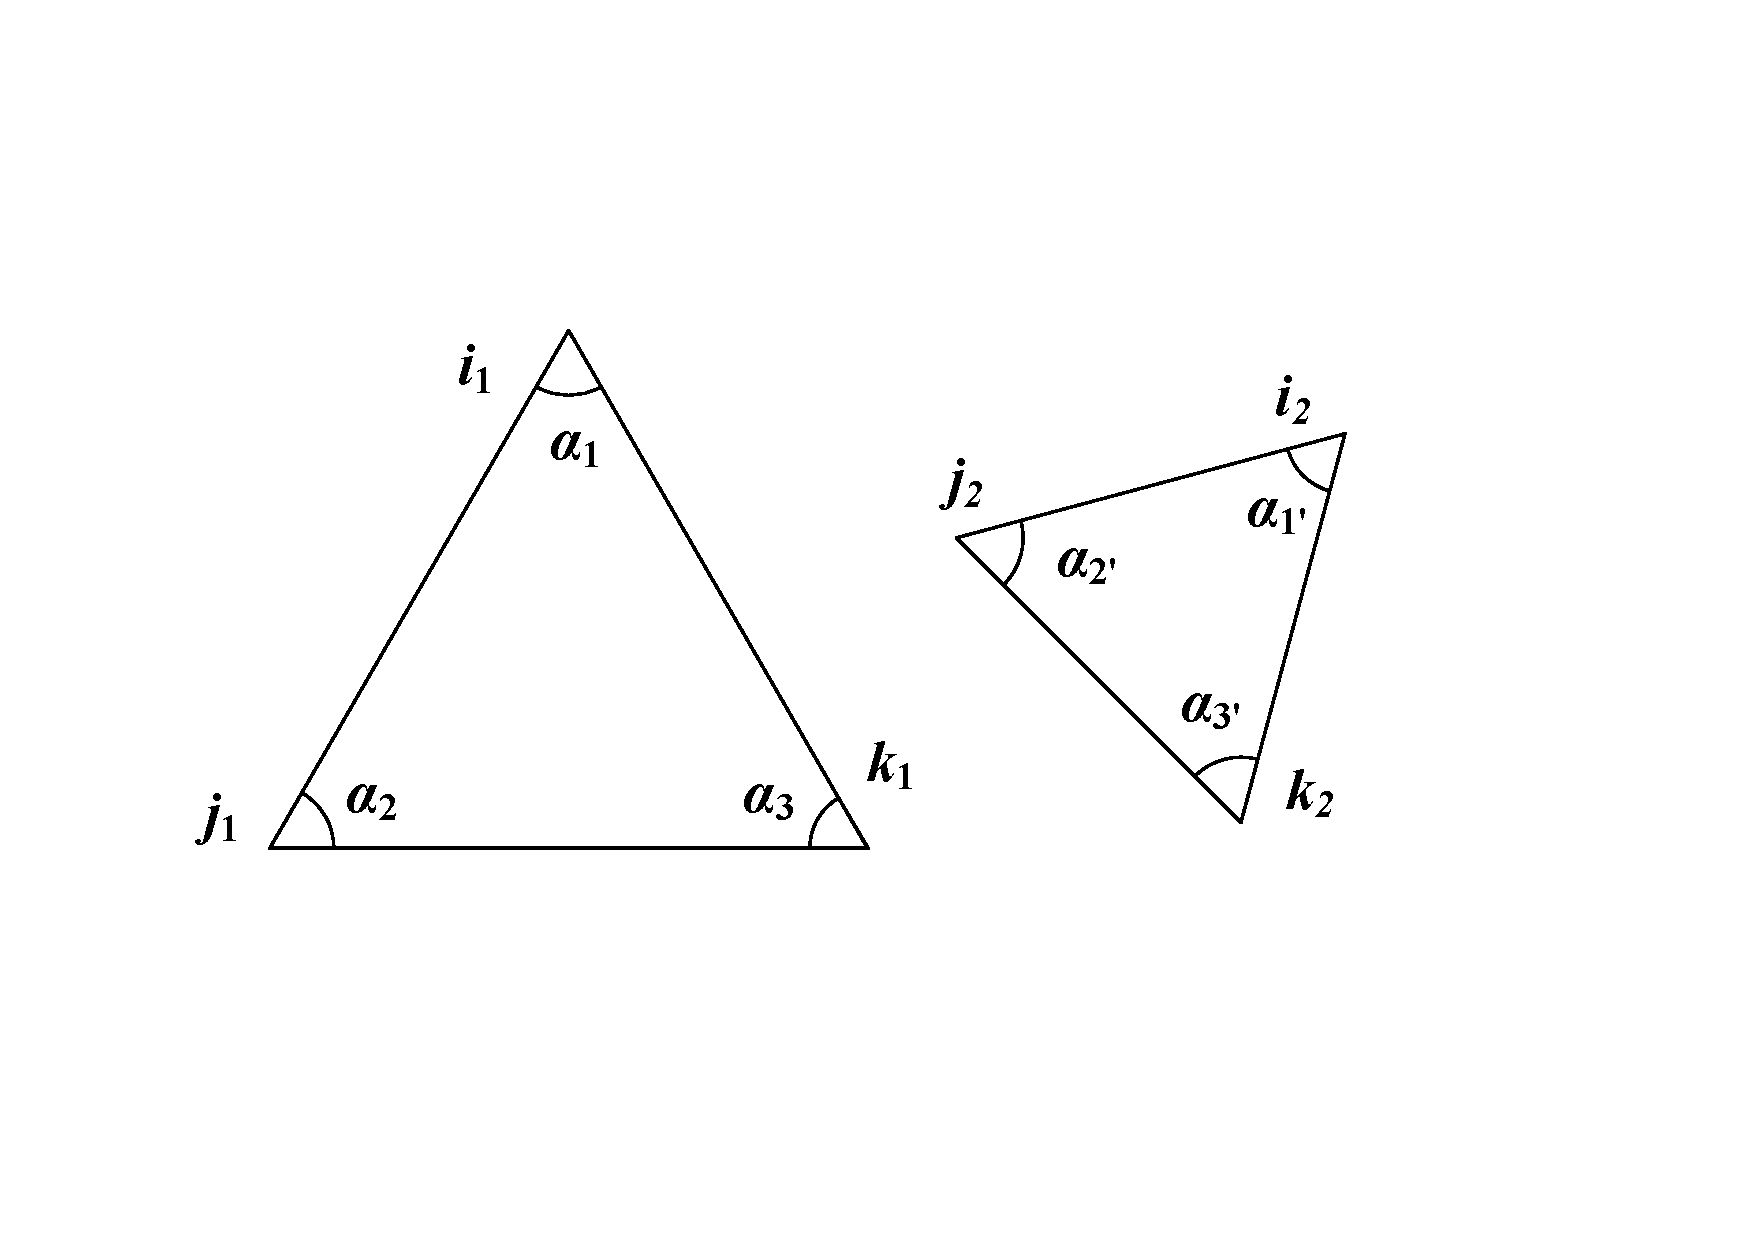
\includegraphics[height=30mm]{thirdorderpotentials.pdf}
  \caption{Third-order potential (triangle).}
  \label{fig:side:thirdorder}
 \end{minipage}%
 \begin{minipage}[!ht]{0.5\linewidth}
  \centering
  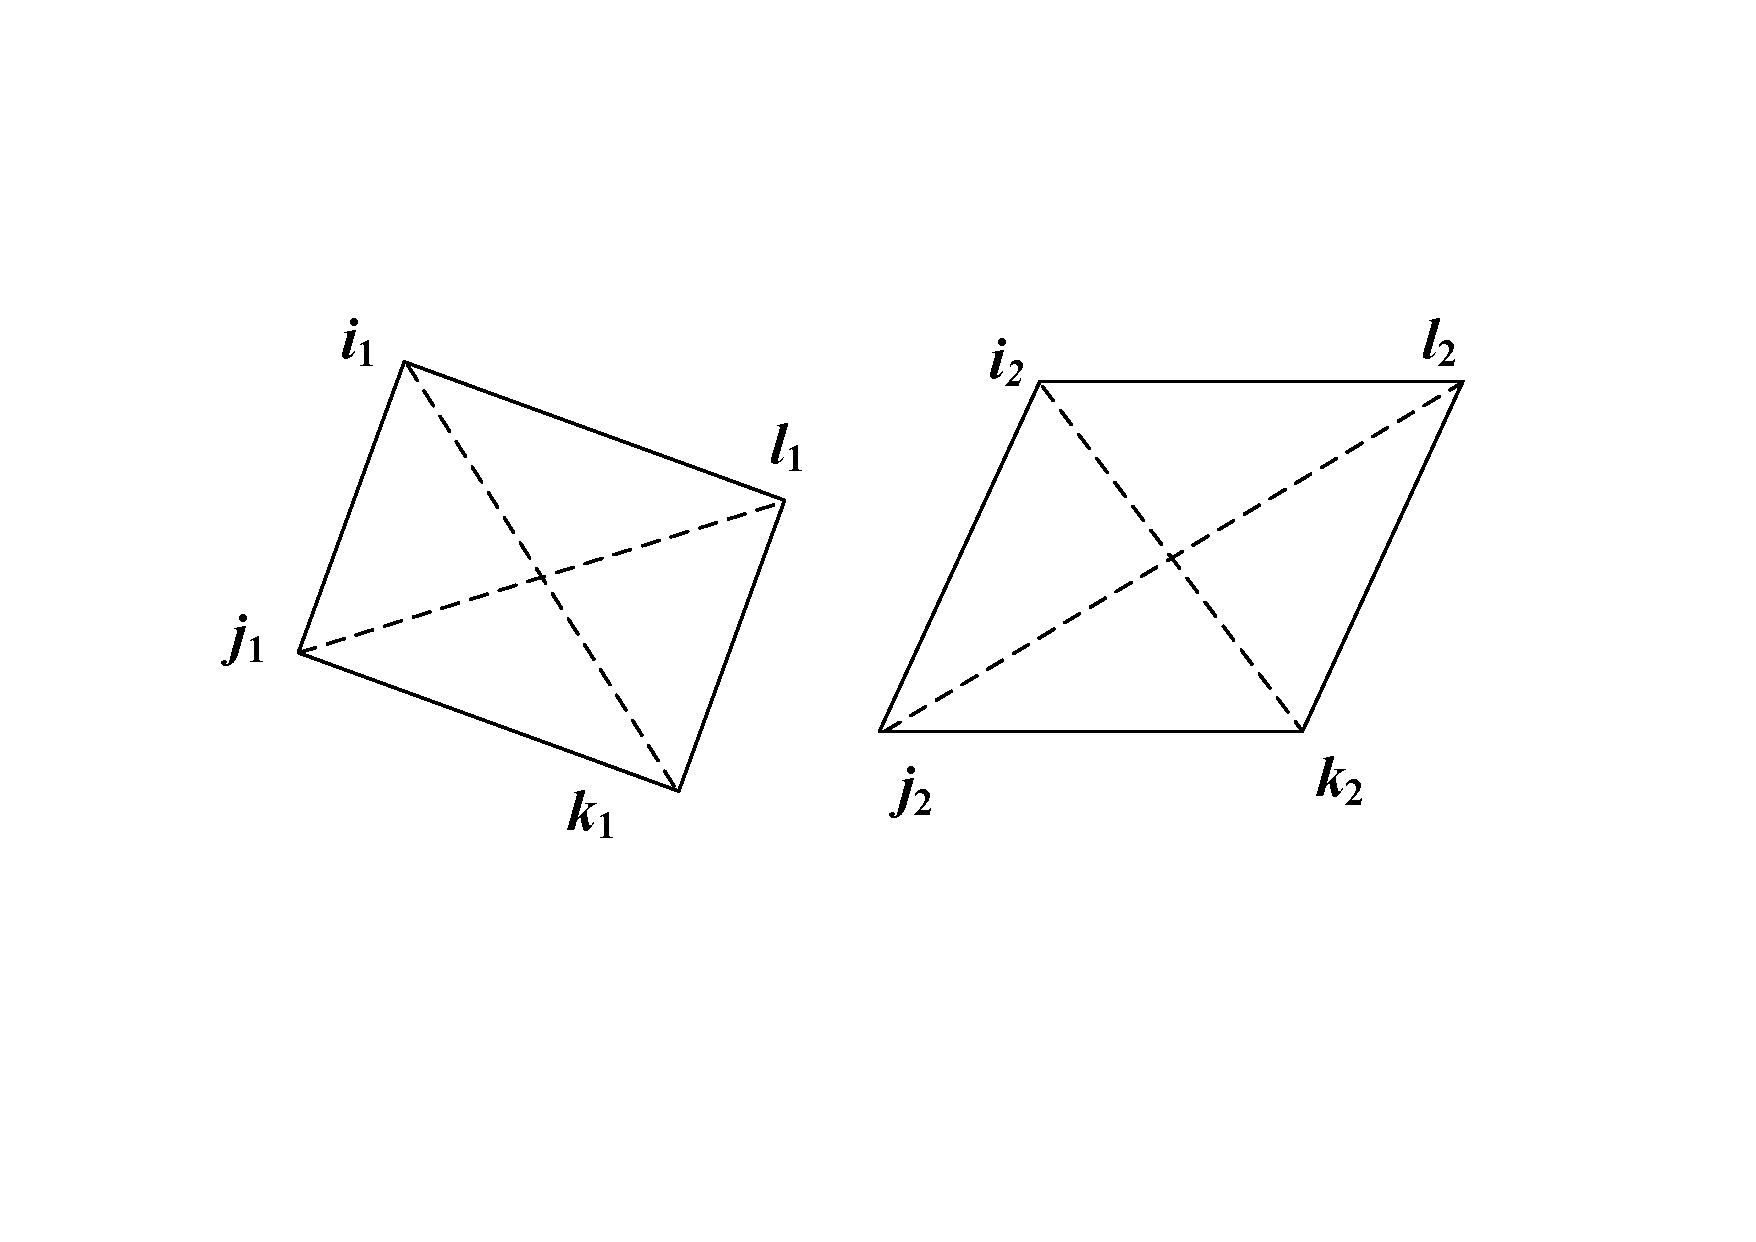
\includegraphics[height=31mm]{fourthorderpotentials.pdf}
  \caption{Fourth-order potential (quadrangle).}
  \label{fig:side:fourthorder}
 \end{minipage}
 \vspace{-4ex}
\end{figure*}

Different higher-order potentials are appropriate for different applications.
Here we give two higher-order potentials, one possessing invariance under similarity transformations (based on triangles) and the other possessing affine invariance (based on quadrilaterals), these kinds of
invariance being useful for many correspondence problems in geometric computing.
The potentials are based on a Gaussian kernel which guarantees the tensor elements are non-negative and invariant to any permutation of the input assignments.

First we restate a well-known~\cite{Duchenne_etal09,Chertok10} third-order geometric-similarity invariant potential $\phi_3$ linking two feature tuples, each having three features.
Similarity of triangles formed by three points corresponds to invariance under scaling, rotation and translation---interior angles do not change.
Thus $\phi_3$ can be defined in terms of differences of corresponding interior angles:
%
\begin{eqnarray}
\phi_3(i,j,k)&=&\phi_3(\{i_1,i_2\}, \{j_1,j_2\}, \{k_1,k_2\})\nonumber\\
&=&\exp(-1/\varepsilon^2\sum\nolimits_{(l,l^{'})}\lVert \alpha_l- \alpha_{l^{'} } \lVert^2 )
\end{eqnarray}
where $\varepsilon > 0$ is the is the kernel bandwidth, and $\{\alpha_l\}_{l=1}^3$  and $\{\alpha_l^{'}\}_{l^{'}=1^{'}}^{3}$ are the angles triangles formed by feature triples $(i_1,j_1,k_1)$ and $(i_2,j_2,k_2)$: see Fig.\ref{fig:side:thirdorder}. Each point corresponds to one interior angle.
%

Feature image matching under  more general affine transformations is also a common problem,
so here we introduce a new fourth-order potential $\phi_4$ which is affine-invariant, linking feature tuples with four features each.
We use affine invariance of the ratio between two closed areas to define $\phi_4$ as:
%
\begin{eqnarray}
\phi_4(i,j,k,l)&=&\phi_4(\{i_1,i_2\}, \{j_1,j_2\}, \{k_1,k_2\}, \{l_1,l_2\}) \nonumber \\
&=&\exp(-1/\varepsilon^2\sum\nolimits_{(l,l^{'})}\lVert \delta_l- \delta_{l^{'} } \lVert^2 )
\end{eqnarray}
where $\{\delta_l\}_{l=1}^4$  and $\{\delta_l^{'}\}_{l^{'}=1^{'}}^{4^{'}}$ are the ratios between the area of one triangle formed by three feature points and the area of the quadrilateral formed by all four feature points, so
$\delta_1=S_{\triangle i_1 j_1 k_1}/S_{\square i_1 j_1 k_1 l_1}$, $\delta_2=S_{\triangle j_1 k_1 l_1}/S_{\square i_1 j_1 k_1 l_1}$, $\delta_3=S_{\triangle i_1 k_1 l_1}/S_{\square i_1 j_1 k_1 l_1}$, $\delta_4=S_{\triangle i_1 j_1 l_1}/S_{\square i_1 j_1 k_1 l_1}$,
and similarly for the other quadrilateral.
%%%RRM better to use A for area, not S

We will use these two higher-order potentials to evaluate our algorithm.

%-------------------------------------------------------------------------
\subsection{Sampling strategy}
\label{subsec:sampling}

Given two feature sets $P_1$ and $P_2$ with $N_1$ and $N_2$ features respectively,
a potential element may be obtained by using two feature tuples sampled from each feature set separately.
For $N$th-order matching, a naive way to construct the potential elements is as follows:
first find all feature tuples for $P_1$ and $P_2$, as $F_1$ and $F_2$; then $\forall (f_{i_1}^1, f_{i_2}^1, \cdots, f_{i_N}^1)\in F_1$,
calculating the potentials for $(f_{i_1}^1, f_{i_2}^1, \cdots, f_{i_N}^1)$ with all feature tuples in $F_2$.
This naive method is very expensive, which is why sampling is used.
Choice of feature tuples to calculate the potentials directly determines the size $|\theta_N\|$ and influences the matching accuracy.
Different sampling strategies can be chosen for different applications,
using random sampling for general feature correspondence problems where there is no guidance to provide a better sampling method.

Here we use a random sampling approach. In order to cover all features in $P_1$ in $F_1$,  we repeatedly take one feature as a required element,
and then  randomly choose $t_1$ feature tuples containing thise required element.
We repeat this process until all features in $P_1$ have been chosen once as a required element.
We do the same for $P_2$. We now have two feature-tuple sets for $F_1$ and $F_2$, containing $N_1 t_1$ and $N_2 t_2$ feature tuples separately.

Now, $\forall (f_{i_1}^1, f_{i_2}^1, \cdots, f_{i_N}^1)\in F_1$, we find the $k$ most similar features in $F_2$ to build $k$ potential elements as $\phi_i^k$.
Combining all the potential elements obtained, we form the desired potential element set $\theta_N = \{\phi_i^k\}_{i=1}^{N_1 t_1}$, with the size $|\theta_N| = N_1 t_1 k$.
The parameters $t_1, t_2$ and $k$ must be chosen according to the size of the feature sets. In practice for two point sets each with a hundred points, this approach works well when $t_1 \approx t_2 \approx 50$ and $k \approx 300$ for third-order or fourth-order matching.
The sampling cost is $O(n\, t\,  k\log n)$, where $n=\max(N_1, N_2), t=\max(t_1, t_2)$.

The most important part of the  process is to use the supersymmetry of the affinity tensor.
An $N^{th}$-order supersymmetric affinity tensor must satisfy:
\begin{eqnarray}
\label{equ:noredun}
\forall (i_1,i_2,\cdots,i_N),(j_1,j_2,\ldots,j_N) \in \theta_N,\nonumber\\(i_1,i_2,\cdots,i_N)\neq\Omega(j_1,j_2,\cdots,j_N)
\end{eqnarray}
where $\Omega$ is an arbitrary permutation.
%%%RRM I dont understand the above expression. There is no quantity being considered.
%%%RRM Your notation needs to express that elements not meeting this are 0.
Thus, we use a sampling constraint that the sets of feature tuples $F_1$ and $F_2$ obtained from the sampling process, should have no repetition, in the sense that
\begin{eqnarray}
\label{equ:noredun2}
\forall (f_{i_1}^1,f_{i_2}^1,\cdots,f_{i_N}^1),(f_{j_1}^1,f_{j_2}^1,\cdots,f_{j_N}^1) \in F_1,\nonumber\\ (f_{i_1}^1,f_{i_2}^1,\cdots,f_{i_N}^1)\neq\Omega(f_{j_1}^1,f_{j_2}^1,\cdots,f_{j_N}^1)
\end{eqnarray}
\begin{eqnarray}
\label{equ:noredun3}
\forall (f_{i_1}^2,f_{i_2}^2,\cdots,f_{i_N}^2),(f_{j_1}^2,f_{j_2}^2,\cdots,f_{j_N}^2) \in F_2,\;\nonumber\\ (f_{i_1}^2,f_{i_2}^2,\cdots,f_{i_N}^2)\neq\Omega(f_{j_1}^2,f_{j_2}^2,\cdots,f_{j_N}^2)
\end{eqnarray}
%%%RRM Notation here also needs making clearer
and $\Omega$ is arbitrary permutation.
This sampling constraint eliminates overlaps that may appear in the potential elements $\theta_N$.

When $N_1$ is not equal to $N_2$ (suppose $N_1<N_2$), we perform sampling as in~\cite{Duchenne_etal09}, using random sampling for $P_1$  but full sampling for $P_2$ (to find all $N_2^N$ feature tuples). However we still use the
sampling constraint for feature-tuple set $F_1$, so our strategy is
different to that in~\cite{Duchenne_etal09}. The process of building the tensor elements is the same to the process stated above when $N_1$ equals to $N_2$. In practice this works well when matching two feature sets with different numbers of features.

Earlier work \cite{Duchenne_etal09,Zass08} also adopted random sampling, but failed to impose any constraint on the sampling process,
leading to the possibility that feature tuples may include repetition.
For example, for third-order matching, it is possible that a feature tuple $(f_{i_1}^1, f_{i_2}^1, f_{i_3}^1)$ may be sampled from $P_1$ and $(f_{i_1}^2, f_{i_2}^2, f_{i_3}^2)$ from $P_2$, and also a feature tuple $(f_{i_1}^1, f_{i_3}^1, f_{i_2}^1)$ sampled from $P_1$ and $(f_{i_1}^2, f_{i_3}^2, f_{i_2}^2)$ from $P_2$. That will create two tensor elements $\phi_3(s_{i_1}, s_{i_2}, s_{i_3})$ with index $(s_{i_1}, s_{i_2}, s_{i_3})$ and $\phi_3(s_{i_1}, s_{i_3}, s_{i_2})$ with index $(s_{i_1}, s_{i_3}, s_{i_2})$, which are the same. However, we just need one tensor element to express the affinity measure on the assignment group $(s_{i_1}, s_{i_2}, s_{i_3})$. This problem not only makes the potential elements redundant but also affects the accuracy of the power iteration, because the numbers of each tensor element may not be equal and some elements may be used more than once during the iteration progress.
Our method reduces the sampling cost, while also improving the accuracy of the power iteration.
